\section{Postscript: Post-Merger Evolution Revised}
\label{sec:c2_postscript}

Since the publication of \citeal{zhu+13}, the work of \cite{ji+13} was published, which is relevant not only because they simulate the post-merger evolution of an equal-mass $0.6-0.6\,\Msun$ remnant, but also because they eschew the use of an $\alpha$-viscosity and instead directly evolve the magnetic field of the merger remnant.  Also published was \cite{rask+14}, which uses the machinery of \cite{schw+12} to generate post-viscous remnant profiles for massive (mostly dissimilar-mass) mergers with $>0.9\,\Msun$ accretors, to determine their nucleosynthetic output if they then experienced a pure detonation.  They do not discuss their viscous simulations in detail.  We have not performed our own post-merger evolution simulations\footnote{We experimented with \flash-based 2.5D simulations that included an $\alpha$-viscosity, but did not follow up with a detailed investigation.}, and use \cite{schw+12} and \cite{ji+13}'s results extensively throughout this thesis - in particular, we reconsidered the simple estimate made in Sec. \ref{ssec:ch2_viscevo_possiblespindown} using \cite{ji+13}'s results when preparing \citeal{zhu+16}.  Since this thesis has no dedicated chapter on post-merger evolution, we expand and update the discussion in Sec. \ref{ssec:ch2_viscevo_possiblespindown} below.

%\cite{shen+12} flesh out the further evolution of \cite{dan+11}'s $0.6 -0.9\,\Msun$ dissimilar-mass merger.  They first use a 1D Lagrangian hydrodynamic simulator with a $\gamma = 5/3$ polytropic equation of state to evolve the (height-integrated) remnant surface density profile under the influence of a uniform $\alpha = 10^{-2}$ viscosity prescription.  This $\alpha$ value is chosen so the system evolves over $t_\mrm{visc} \sim 10^{4}\,\mrm{s}$, roughly consistent with the viscosity arising from either the magnetorotational instability (MRI; \citealt{balbh91}) or (in region where its onset is unfavourable) the Tayler-Spruit dyanamo (eg. \citealt{spru02}).  Material inside of $M_\mrm{enc} = 0.9\,\Msun$ is assumed to remain unchanged.  Note that $\alpha$ is likely to be non-uniform in space and time, as, for example, the Tayler-Spruit dynamo viscosity will not be identical to that of the MRI, but \cite{shen+12} argue this will only change the details of the evolution -- the qualitative results remain unchanged so long as the viscous timescale falls between the dynamical and thermal ones.  They find -- as expected from viscous evolution -- evolution toward a shear-free solid body rotation, with the sub-Keplerian disk converted to a thermally supported, near-virial, tenuous atmosphere.  This atmosphere ($\rho \lesssim 10^4\,\gcc$, $T \sim 10^9\,\mrm{K}$) is radiation-dominated, and so has a near-Eddington luminosity.  

%  Since the $0.6 - 0.9\,\Msun$ merger has a cold core with little rotational support, the loss of this support does not heat it substantially; the hottest point in the remnant is instead a ``hot ring'' residing at the boundary between the $0.9\,\Msun$ accretor and disrupted donor material, formed by shock-heated donor material falling onto the accretor.

%\cite{schw+12} replace \cite{shen+12}'s Lagrangian solver with the \textsc{ZEUS-MP2} \citep{haye+06} Eulerian hydrodynamics code, modified with the Helmholtz \citep{timms00} equation of state, a stress-tensor term with a dynamic viscosity coefficient given by $\alpha = 3\times10^{-2}$ ($\alpha = 10^{-4} - 10^{-1}$ lead to qualitatively similar end results) and a simplified five-isotope nuclear network.  They simulate eight dissimilar-mass merger remnants (from \citealt{dan+11}), including two CO-CO ones, and confirm \cite{shen+12}'s qualitative results, most notably that a combination of spin-down and viscous heating converts the rotationally-supported outer layers of the remnant to a spherically symmetric, thermally-supported and convectively unstable hot atmosphere.  For their fiducial $0.6 - 0.9\,\Msun$, spin-down increases the hot ring's temperature by a factor of $\sim1.5$, and density by a factor of $\sim3$, enough to push it above the carbon ignition line.  The other remnants they consider are either remnants of He-CO mergers with extreme mass ratios, those of low-mass He-He mergers, or massive, $\gtrsim1.7\,\Msun$ ones.  The results of these systems are very similar to their fiducial one, except for the contribution of He nuclear burning to the temperature structure of the spun-down remnant for He-CO remnants.

\cite{ji+13} implements their magnetohydrodynamic simulation using the Eulerian grid code \flash\ \citep{fryx+00} and with the $0.6 - 0.6\,\Msun$ remnant of \citeal{loreig09} for initial conditions.  Like \cite{schw+12}, they utilize a 2.5D axisymmetric grid, where a 2D grid extends along $\hat{r}$ and $\hat{z}$ (\cite{schw+12} use a $\hat{r}-\hat{\theta}$ spherical grid instead), while $\hat{\phi}$ quantities remain constant for all $\phi$, and the Helmholtz EOS.  Since \citeal{loreig09}'s remnants are unmagnetized, they artificially insert a purely poloidal magnetic field whose strength is $\sim10^8\,\mrm{G}$ in the remnant disk, and $\lesssim10^5\,\mrm{G}$ in the core (they determine their results are robust to changing initial field strength and spatial resolution by factors of 2).  They advance their simulation to $2\times10^4\,\mrm{s}$, comparable to the completion times in \cite{schw+12}.  They find that the magnetorotational instability (MRI) acts on the differentially rotating portions of the remnant to greatly amplify the field over several hundred seconds, resulting in an equilibrium field with a peak strength of $\sim10^9\,\mrm{G}$ in the disk and $\gtrsim10^{10}\,\mrm{G}$ in the core, as well as a total magnetic energy of $\sim10^{48}\,\mrm{erg}$, on part with the differential rotation energy of the system (see Ch. \ref{ch:ch4}).  This field produces Maxwell stresses that are roughly equivalent to $\alpha \sim 10^{-2}$ viscosity, facilitating global outward angular momentum transport like in \cite{schw+12}.  It also generates a hot, magnetized corona by displacing disk material through magnetic buoyancy, and a binconal outflow along the remnant's rotational axis.  These outflows eject $10^{-3}\,\Msun$ of material at roughly twice the local escape speed (of $\sim1600\,\mrm{km}\psec$).  

Much like \cite{schw+12}, the remnant loses most of its rotational support and evolves toward a spherically symmetric state with a dense, degeneracy-supported core and a more tenuous thermally-supported envelope.  By the end of the simulation $\sim0.08\,\Msun$ of material either resides in the magnetically dominated corona or is outfluxed from the simulation domain, leaving $1.12\,\Msun$ remaining in the remnant -- though this does not distinguish between the core and envelope.  Accretion onto and loss of rotational support within the core leads to its center being compressionally heated by a factor of $\sim2.5$ in density and $\sim2$ in temperature.  As their initial conditions are a factor of $\sim2$ hotter than our equivalent $0.6 - 0.6\,\Msun$ remnant (Sec. \ref{ssec:c2_compwithloreig}), this additional compression ignites central nuclear fusion.

How do \cite{ji+13}'s results, alongside \cite{schw+12}'s, compare to our simple estimates of viscous evolution in Sec. \ref{ssec:ch2_viscevo_possiblespindown}?  The most relevant quantities we need are the density and temperature at the center and at the hottest point of the post-viscous remnant, to determine whether carbon fusion ignites under highly degenerate conditions and the amount of material that remains a part of the dense, degeneracy-dominated remnant core.  The latter is important for comparing against simmering WDs in Chapter \ref{ch:ch6}.  As noted in Sec. \ref{ssec:ch2_viscevo_possiblespindown}, we estimate the hottest point within our $0.6-0.9\,\Msun$ remnant increases by a factor of $2.5$ in density and $1.6$ in temperature, very similar to \cite{schw+12}'s results.  The central density of their remnant is $1.75\times10^7\,\gcc$ at the start of viscous evolution \citep{dan+11} and $2.8\times10^7\,\gcc$ at the end -- an factor of $1.6$ increase, while we find a factor of $2.0$.  We tend to estimate much larger amounts of compressional heating for similar-mass systems, however, finding that the $0.6 - 0.6\,\Msun$ one increases its central density and temperature by a factor of $6.6$ and $2.7$, respectively, substantially larger than the $\sim2.5$ and $\sim2$ found by \cite{ji+13}.  Similarly, \cite{rask+14} find the central density of their $1.0-1.0\,\Msun$ remnant increases from $7.1\times10^7\,\gcc$ to $2.4\times10^8\,\gcc$, a much smaller compression than the factor of $\sim10$ we find.  This is likely because our simple estimate assume all rotational energy is deposited as heat solely in the outermost regions of the remnant, while in reality remnants, particularly those of similar mass, are rotationally supported throughout and thus will likely also be heated throughout during viscous evolution, reducing the amount of core compression.  We also note \cite{ji+13}'s remnant also has not fully lost core rotational support at the end of their simulation, with $\Omegac$ still $\approx 0.15\,\psec$.\footnote{We do not know if the same is true for \cite{rask+14}'s simulations.  \cite{ji+13} additionally note the central temperature at the end of evolution has not converged, increasing by $\sim20$\% with spatial resolution.}  We therefore can make reasonable estimates for dissimilar mass systems, but overestimate by a factor of a few the degree of compression and heating in similar-mass ones.

%There are unfortunately no other systems we can directly compare to, but we are able to use more of \cite{schw+12}'s results to determine the mass of the post-viscous core. 

% The central density of schw+12's 0.6 - 0.9Msun remnant comes from Table 1 of dan+11; the spun-down value comes from Table 3 of schw+12.  For the 0.6 - 0.6 system, we use the central term in the xy-plane temperature-density relationship ("crho" and "cT" if using GitHubTemp/PaperRunaway/papercalc_other.py) rather than the max values.

\begin{figure}
\centering
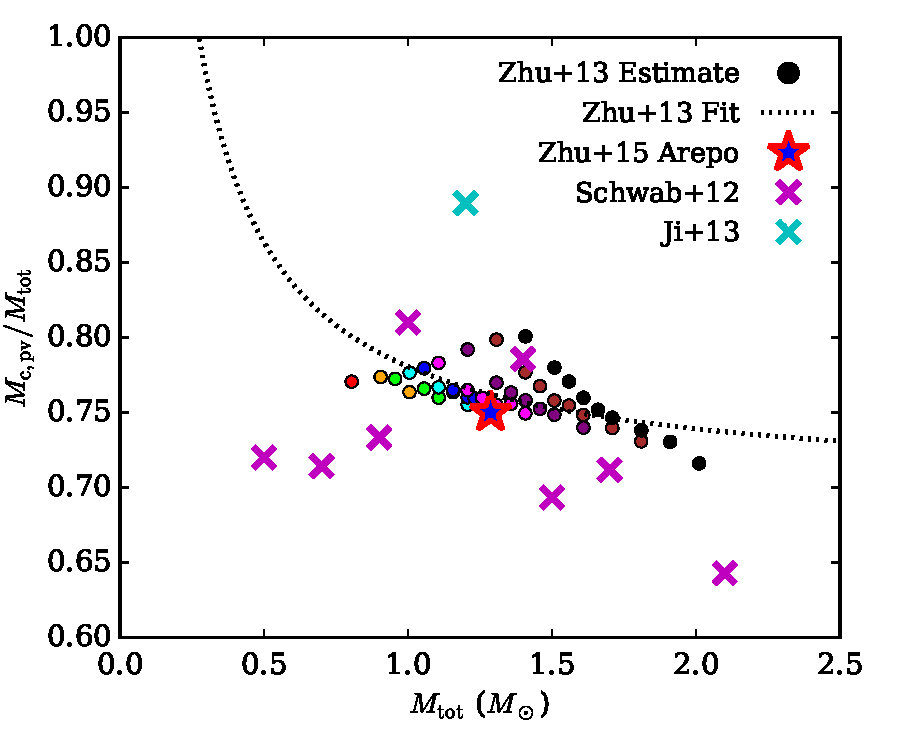
\includegraphics[angle=0,width=0.6\columnwidth]{chapter2_zhu+13/figures/c2a_mcpv.pdf}
\caption{Post-viscous degenerate core mass \Mcpv, estimated using the simple viscous evolution prescription in Sec. \ref{ssec:ch2_viscevo_possiblespindown}, as a function of remnant total mass \Mtot, for the simulated systems of \citeal{zhu+13} (points; colors have the same meaning as in Fig. \ref{fig:c2_willitexplode}) and the $0.625 - 0.65\,\Msun$ remnant from the \arepo\ MHD simulation (Ch. \ref{ch:ch4}; red-blue star).  Also plotted are estimates of \Mcpv\ from \citeauthor{schw+12} (\citeyear{schw+12}; using $M_\mrm{c} + M_\mrm{tp}$ in their Table 3) and \citeauthor{ji+13} (\citeyear{ji+13}; estimated from integrating its spherical density profile to $r = 2\times10^9\,\mrm{cm}$).  The dotted line is a best fit to the \citeal{zhu+13} points.}
\label{fig:c2a_mcpvvsmtot}
\end{figure}

In our simple estimate, the mass of the post-viscous core, \Mcpv, is given by the mass of the spherically symmetric hydrostatic model representing the spun-down remnant (Sec. \ref{ssec:ch2_viscevo_possiblespindown}).  In Fig. \ref{fig:c2a_mcpvvsmtot}, we plot this mass versus the total mass of the merging binary, finding that to first order

\eqbegin
\Mcpv = 0.70\Mtot + 0.08\,\Msun,
\label{eq:c2a_mfit}
\eqend

\noindent (\Mcpv\ also has a weak inverse dependence on mass ratio \qm).  We also perform our estimate on the $0.625 - 0.65\,\Msun$ remnant from our \arepo\ \citep{spri10} MHD simulation in Ch. \ref{ch:ch4}, and find little difference from its \gasoline\ counterpart.  For \cite{schw+12}, \Mcpv\ can be estimated from the combined mass of the core and isothermal region ($M_\mrm{c} + M_\mrm{tp}$ in their Table 3), which overall follow the slope of Eqn. \ref{eq:c2a_mfit} but tend to be $\sim0.1\,\Msun$ below it.  For \cite{ji+13}, we estimate (from their Fig. 1) the spherical boundary between the dense core and tenuous envelope to be $r \approx 1.5\times10^9\,\mrm{cm}$; \Mcpv\ can then be estimated by determining the enclosed mass, which is $1.07\,\Msun$ (Suoqing Ji and Robert Fisher private communication), or $\sim0.15\,\Msun$ above Eqn. \ref{eq:c2a_mfit}'s estimate.  Our estimate therefore only roughly reproduces (with errors of $\sim0.1\,\Msun$) the amount of mass remaining in the post-viscous core, partly because the assumption that material not in the core is marginally bound with $E = 0$ is overly simplistic, and partly because \Mcpv\ is somewhat difficult to define in a system that may be supported by both degeneracy and thermal pressure.

%and the amount of compressional heating the core experiences

%Our estimates' tendency to overestimate \Mcpv\ is likely because it assumes material not part of the remnant core is marginally bound with $E = 0$, leading to underestimation of the hot envelope mass.  Therefore our simple estimate overall does roughly produce the amount of mass remaining in the post-viscous core, and the amount of compressional heating the core experiences.(at least for dissimilar mass systems) attached to the degenerate core following spin down, but in detail tends to overestimate both effects.

For those systems that do not ignite nuclear fusion during the viscous phase, their next stage of evolution involves entropy being transported via radiative diffusion throughout and away from the remnant.  Since the remnant hot envelope ($\rho \lesssim 10^4\,\gcc$, $T \sim 10^9\,\mrm{K}$) is radiation-dominated, it has a near-Eddington luminosity, and thermal evolution will occur over a timescale \citep{shen+12}

\eqbegin
t_\mrm{therm} \sim E_\mrm{th, envelope}/L_\mrm{edd} \sim 10^4\,\mrm{yr}.
\eqend

\noindent (For those systems that do ignite fusion, the nuclear runaway time is $\lesssim10^2\,\mrm{yr}$, so this evolution will only occur to a very limited extent.)  \cite{shen+12} simulates this phase of thermal evolution using the \mesa\ \citep{paxt+11, paxt+13, paxt+15} 1D quasi-hydrostatic stellar evolution code, but use an artificial stellar profile that approximates their $0.6-0.9\,\Msun$ post-viscous remnant.  Notably, they set the peak temperature at the base of the hot envelope (at $m \sim 0.9\,\Msun$) below the carbon ignition line.  They find the entropy from the remnant interior diffuses outward over $\sim10^4\,\mrm{yr}$, leading to the further compression and heating of the interior until carbon fusion ignites at the (non-degenerate) base of the envelope.  Meanwhile, convection rapidly redistributes entropy to much of the envelope, expanding it until its photosphere reaches $10^{12}-10^{13}\,\mrm{cm}$, comparable to giant stars.  They predict that their remnant will be converted into an ONe WD, much like in earlier calculations of near-Eddington accretion onto massive WDs (eg. \citealt{saion85}).

More recently, \cite{schw+16} have directly ported their post-viscous $0.6-0.9\,\Msun$ remnant from \cite{schw+12}, and a more massive $0.64-0.96\,\Msun$ one from \cite{rask+14}, into \mesa\ to simulate their thermal evolution.  The peak temperatures of both remnants are already high enough to ignite carbon nuclear fusion at the very start of the simulation; this generates a carbon-burning shell that propagates inward via conduction, reaching the center of the WD in $\sim2\times10^4\,\mrm{yr}$.  The result is a non-degenerate, but still bound, ONe WD, which will subsequently cool through neutrino losses and contract.  For those remnants with masses $\gtrsim1.35\,\Msun$, this contraction leads to off-center \textit{neon} burning to silicon-group elements, and for super-\Mch\ remnants, may even lead to fusion to iron followed by core-collapse into a neutron star.  For substantially sub-\Mch\ remnants that nevertheless ignite non-explosive burning, though, the likely end result is a massive ONe WD.

%\cite{shen+12} simulate their $0.6-0.9\,\Msun$ remnant's thermal evolution in the \mesa\ \citep{paxt+11} 1D quasi-hydrostatic stellar evolution code.  Due to their viscous code using flattened cylindrical coordinates, they cannot directly port its output into \mesa, and instead evolve an artificial stellar profile that approximates the post-viscous remnant.  Notably, they set the peak temperature at the base of the hot envelope below the carbon ignition line.  They find the entropy from the remnant interior diffuses outward over $\sim10^4\,\mrm{yr}$, leading to the further compression and heating of the interior.  After $\sim6000\,\mrm{yr}$, carbon fusion ignites at the (non-degenerate) base of the envelope (at $m \sim 0.9\,\Msun$), though these values are of course dependent on their artificial initial conditions.  Whenever it is ignited, the nuclear burning zone will stably convert carbon into oxygen and neon, and will diffuse into the remnant interior over $10^4\,\mrm{yr}$.  Meanwhile, convection rapidly redistributes entropy to much of the envelope, expanding the envelope until its photosphere reaches $10^{12}-10^{13}\,\mrm{cm}$, comparable to giant stars.  

Thermal evolution of post-viscous remnants that are hottest at their \textit{center} have, to our knowledge, not yet been calculated.  We expect it would be qualitatively similar to the findings of \cite{shen+12} and \cite{schw+16} their dissimilar-mass remnants: a further compression of the interior over $\sim10^4\,\mrm{yr}$, and less heating than if the compression were adiabatic, since radiative and neutrino cooling become significant over these longer timescales.  We thus expect that systems brought to the brink of ignition by viscous spin-down may subsequently ignite due to thermal contraction, though the number of such systems is likely to be small.  Those whose central temperatures are significantly below $6\times10^8\,\mrm{K}$ will cool too much during their compression to ignite, and, since neutrino cooling is density-dependent, may experience off-center ignition instead.

The radiation-dominated envelope alongside the remnant's carbon-oxygen composition, however, suggest that the remnant drives strong winds, complicating the thermal evolution and potentially preventing an AIC \citep{shen+12, schw+16}.  They may also impress the remnant with distinct observational properties, which we discuss in Sec. {\charles XXX}.
